%!TEX root = constraint-layout.tex

% \newcommand{\teaserFigure}{
% 	\teaser{
% 		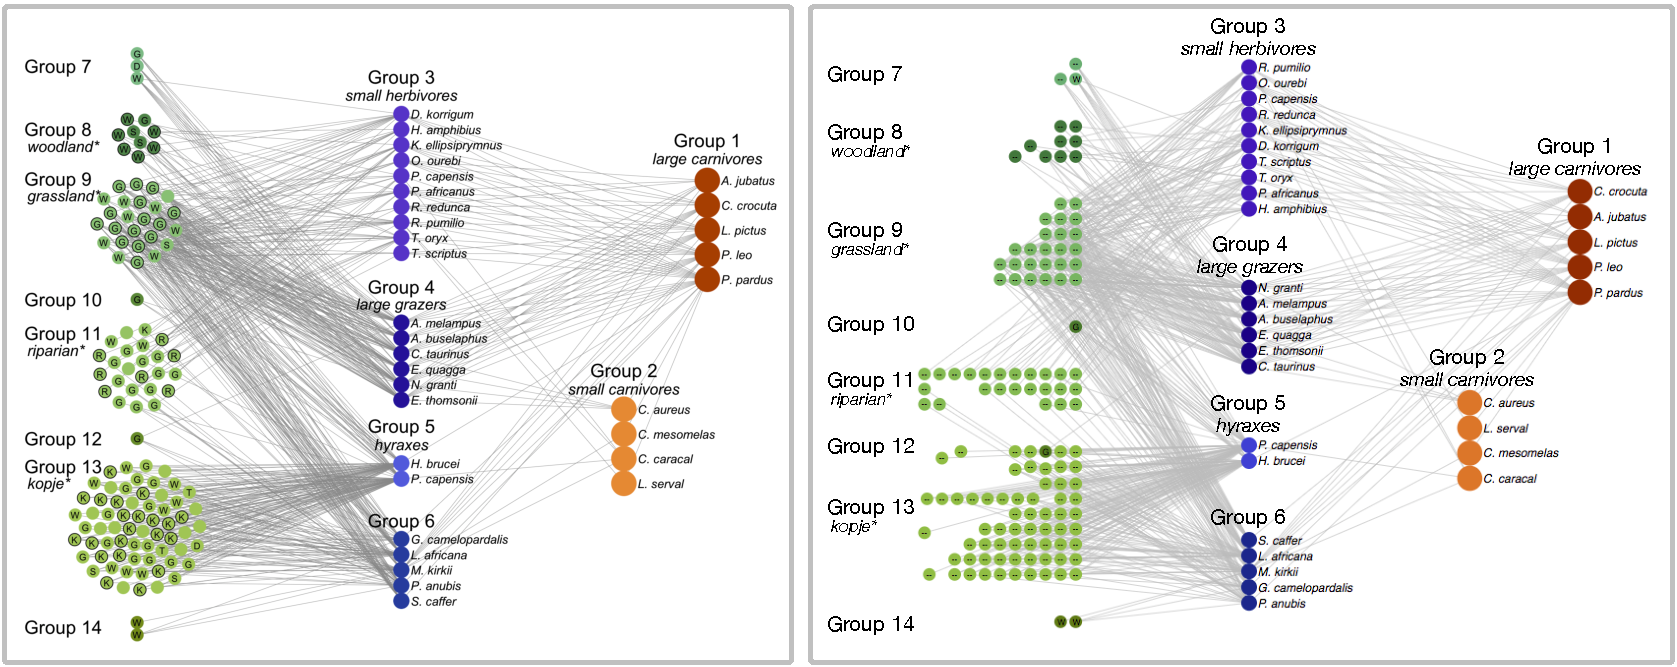
\includegraphics[width=\linewidth]{figures/serengeti-layout.pdf}
% 		\centering
% 	  \caption{\label{fig:teaser}}

% 	}
% }

\newcommand{\serengetiLayoutColumn}{
  \begin{figure}[t!]
    \centering
    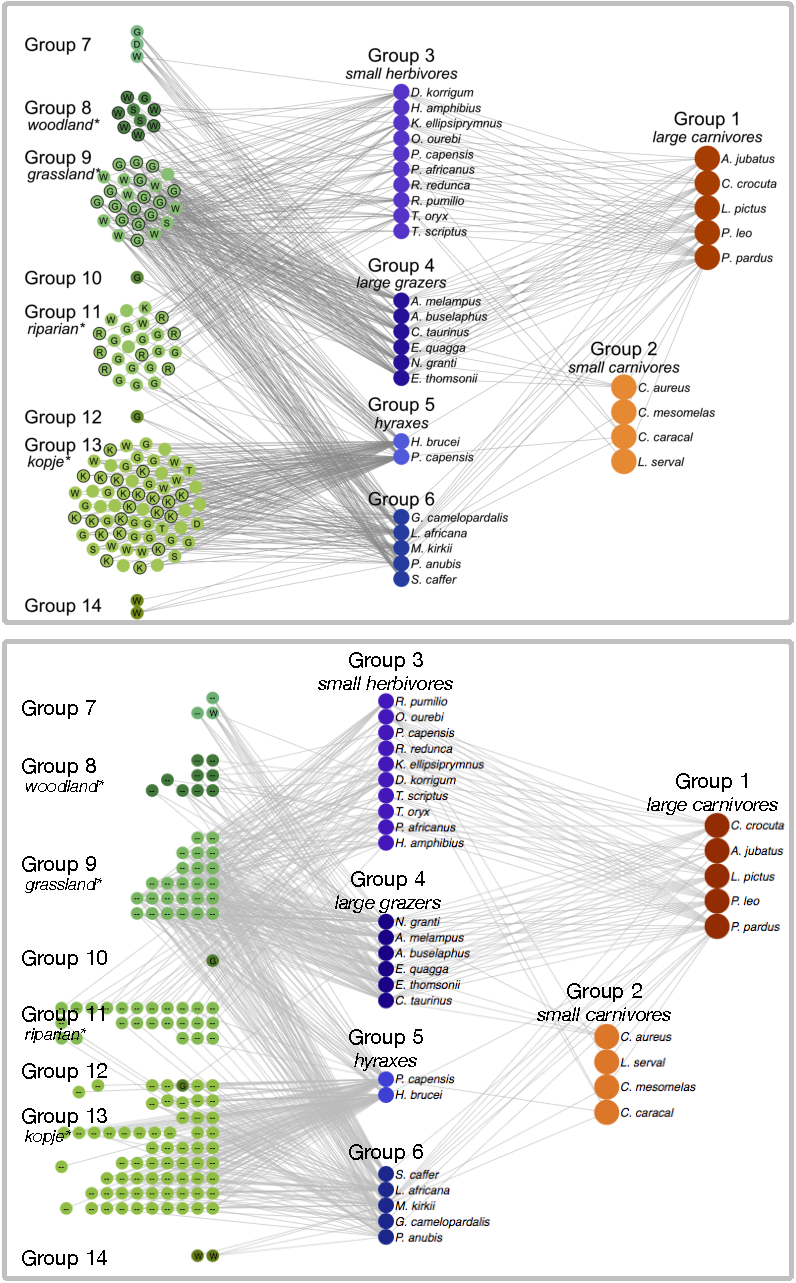
\includegraphics[width=0.81\columnwidth]{figures/serengeti-layout-column.pdf}
    {\caption{\label{fig:serengeti-layout}
    The layout for the Serengeti food web using our constraint language, as compared to Baskerville et al.~\cite{baskerville2011spatial}.}}
    \vspace{-40px}
  \end{figure}
}

%%%%%%%%%%%%%%%%%%%%%%%%%%%%%%%%%%
%%%%%%%%%%%%% Design %%%%%%%%%%%%%
%%%%%%%%%%%%%%%%%%%%%%%%%%%%%%%%%%

\newcommand{\smallTreeExample}{
  \begin{figure}[t!]
    \centering
    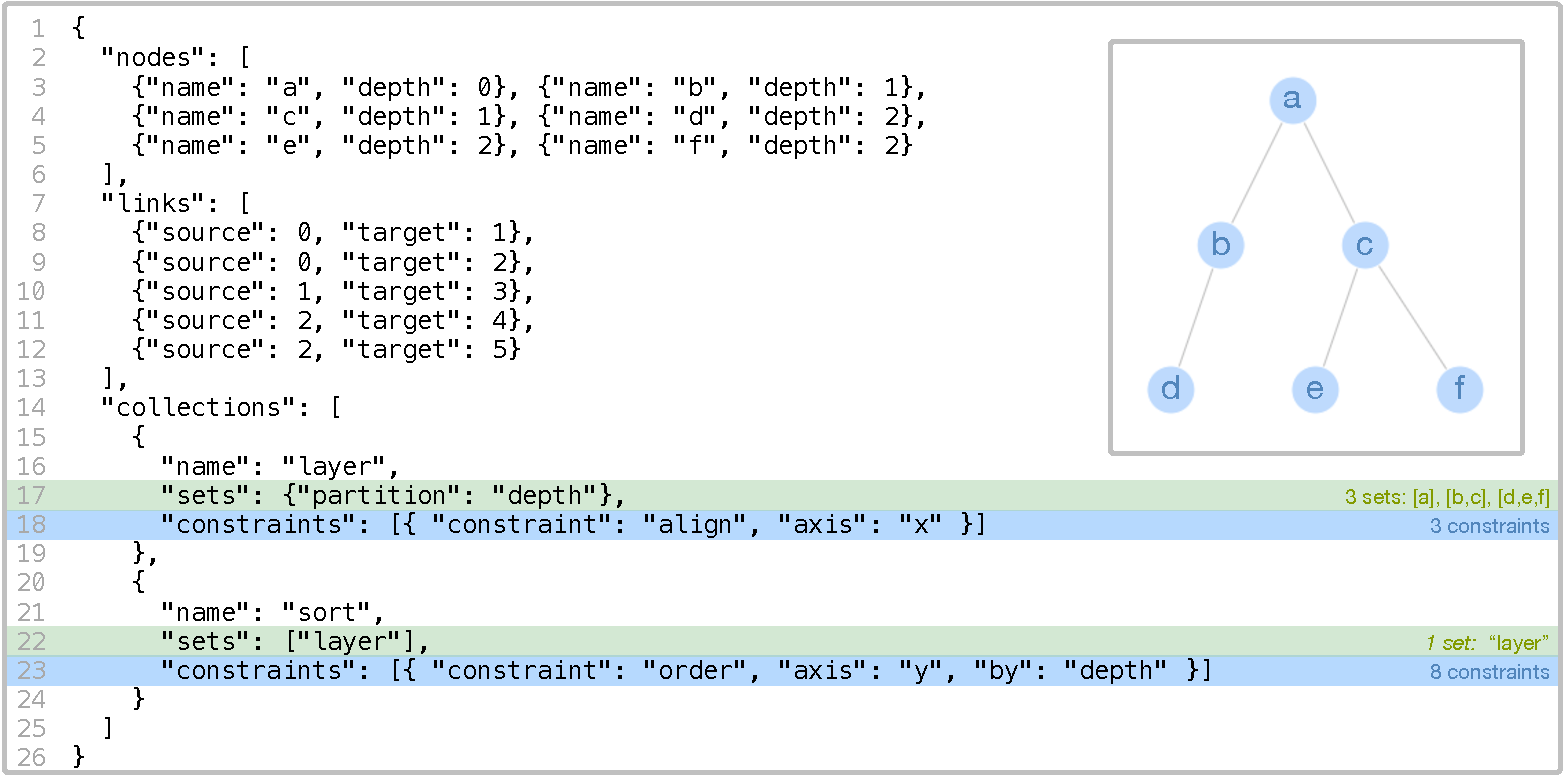
\includegraphics[width=\columnwidth]{figures/small-tree-example.pdf}
      {\caption{\label{fig:small-tree-example} The \projectname specification
      and data for a small tree with six nodes. Nodes are split into sets 
      based on their \texttt{depth} from the root ``\texttt{a}'', and aligned. 
      A new set definition uses composition to include the ``layer'' set
      and the layers are ordered by their depth to form the tree. 
      \feedback{Matt}{Just an idea but maybe write the spec Figure 2. in 
     YAML instead of JSON so its easier to read? Makes your work look better 
     too if the spec looks simpler.} }}
    \vspace{-20px}
  \end{figure}
}

\newcommand{\contradictionExample}{
  \begin{figure}[t!]
    \centering
    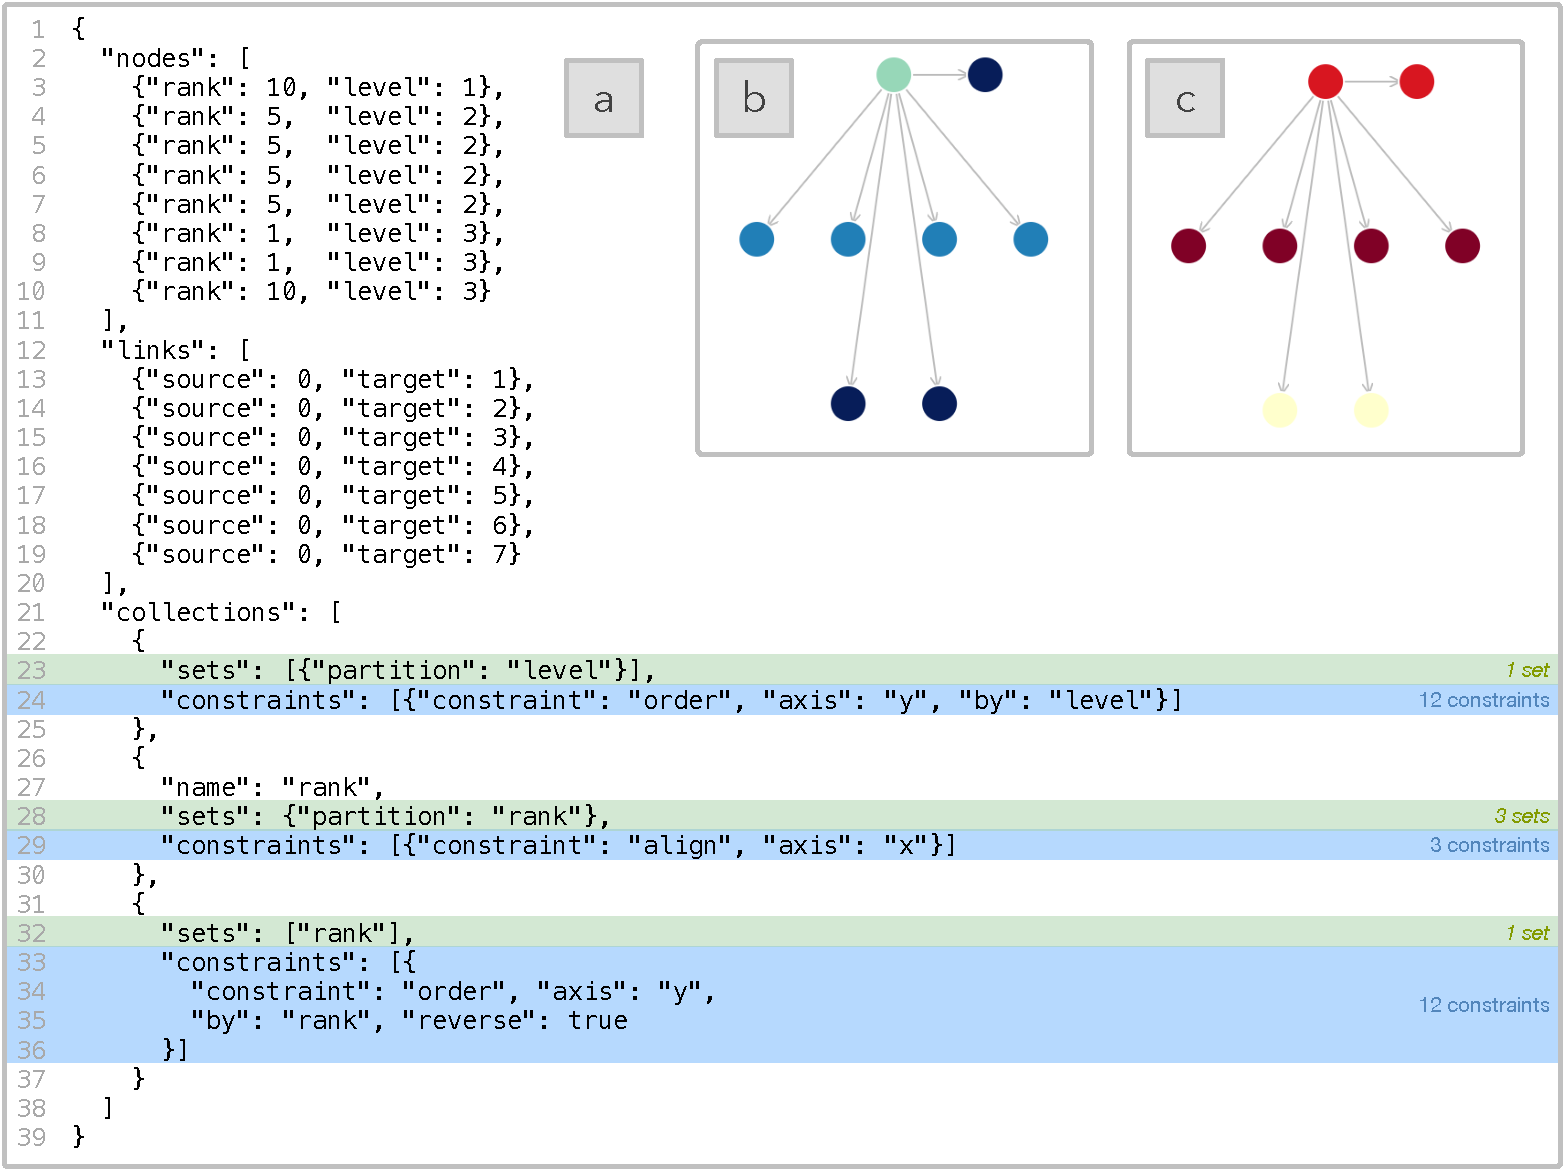
\includegraphics[width=\columnwidth]{figures/contradiction-example.pdf}
      {\caption{\label{fig:contradiction-example} (a) The full \projectname
      specification for a small graph with eight nodes. (b) Nodes are 
      aligned based on their \texttt{rank}, and colored based on their
      \texttt{level}. Two constraints are applied to order the nodes, 
      once by \texttt{level} and once by \texttt{rank}, which produces 
      a contradiction. (c) Nodes are colored based on the amount of error 
      for constraints that are invalid.}}
    \vspace{-20px}
  \end{figure}
}

%%%%%%%%%%%%%%%%%%%%%%%%%%%%%%%%%%
%%%%%%%%% Demonstration %%%%%%%%%%
%%%%%%%%%%%%%%%%%%%%%%%%%%%%%%%%%%

\newcommand{\krugerLayout}{
  \begin{figure}[t!]
    \centering
    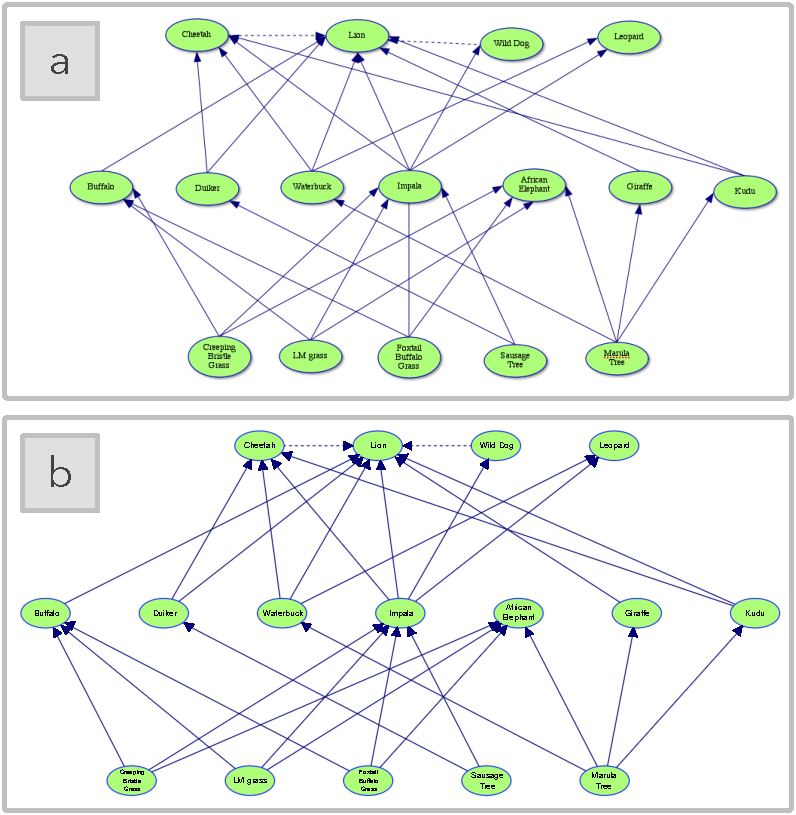
\includegraphics[width=\columnwidth]{figures/kruger-layout.pdf}
    \vspace{-20px} {\caption{
      \label{fig:kruger-layout} A subset of the food web for Kruger 
      National park arranged by trophic level (i.e., carnivore, 
      herbivore, and plant), as seen on the website \cite{kruger2017} 
      and (b) recreated using \projectname.
    }}
    \vspace{-20px}
  \end{figure}
}

\newcommand{\serengetiLayout}{
  \begin{figure*}[t]
    \centering
    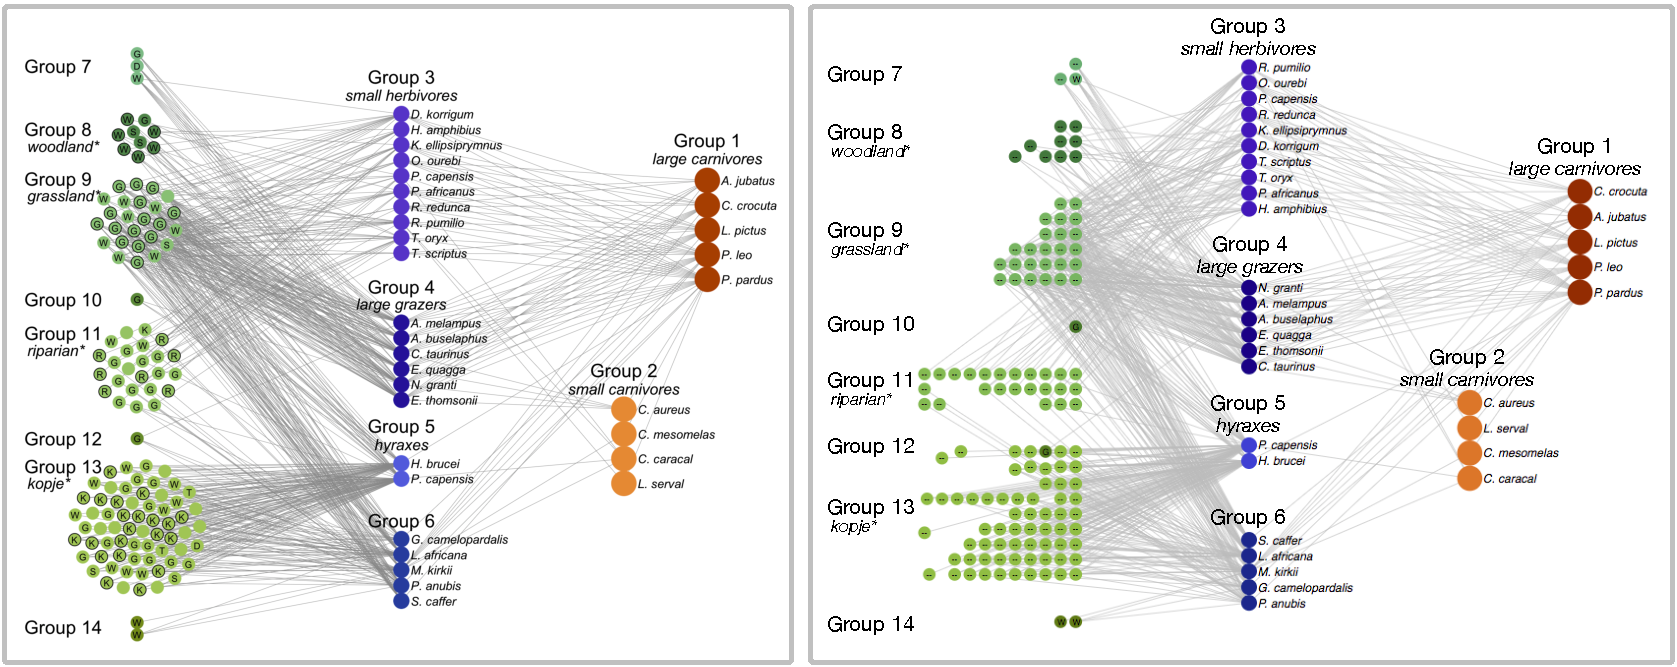
\includegraphics[width=\textwidth]{figures/serengeti-layout.pdf}
    \vspace{-20px} {\caption{\label{fig:serengeti-layout} The layout for
        the Serengeti food web from (a) Baskerville et al.~\cite{baskerville2011spatial}
        as compared to (b) the layout recreated with \projectname.
        Nodes are grouped by trophic level clusters produced from a Bayesian
        analysis method.}}
  \end{figure*}
}

\newcommand{\serengetiSpec}{
  \begin{figure}[h!]
    \centering
    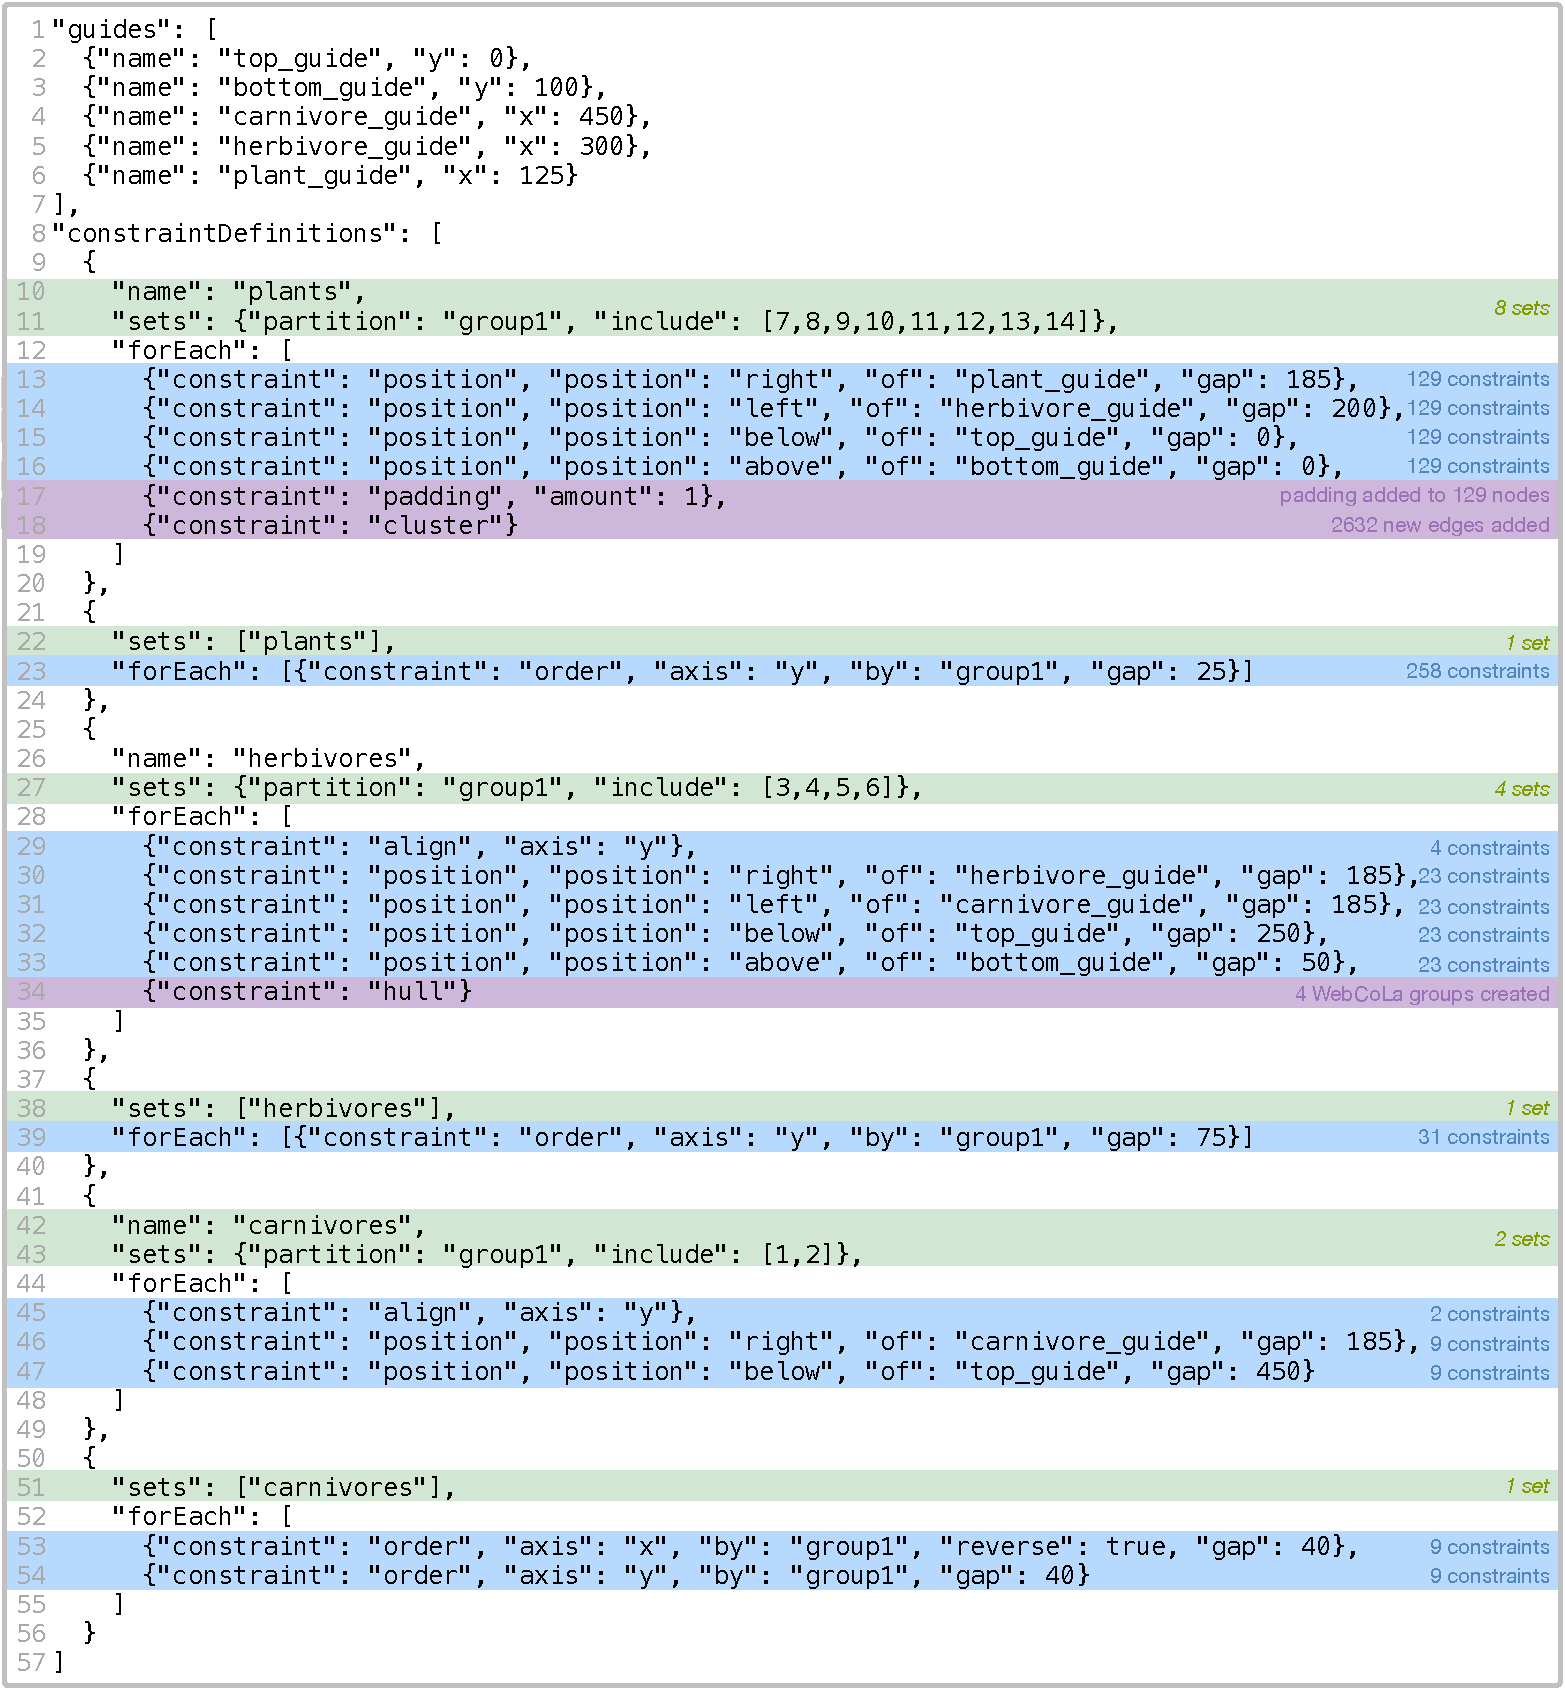
\includegraphics[width=\columnwidth]{figures/serengeti-spec.pdf}
    \vspace{-20px} {\caption{\label{fig:serengeti-spec} The
        \projectname~specification for the Serengeti food web shown in
        Figure~\ref{fig:serengeti-layout}.}}
    \vspace{-10px}
  \end{figure}
}

\newcommand{\syphilisLayout}{
  \begin{figure*}[t]
    \centering
    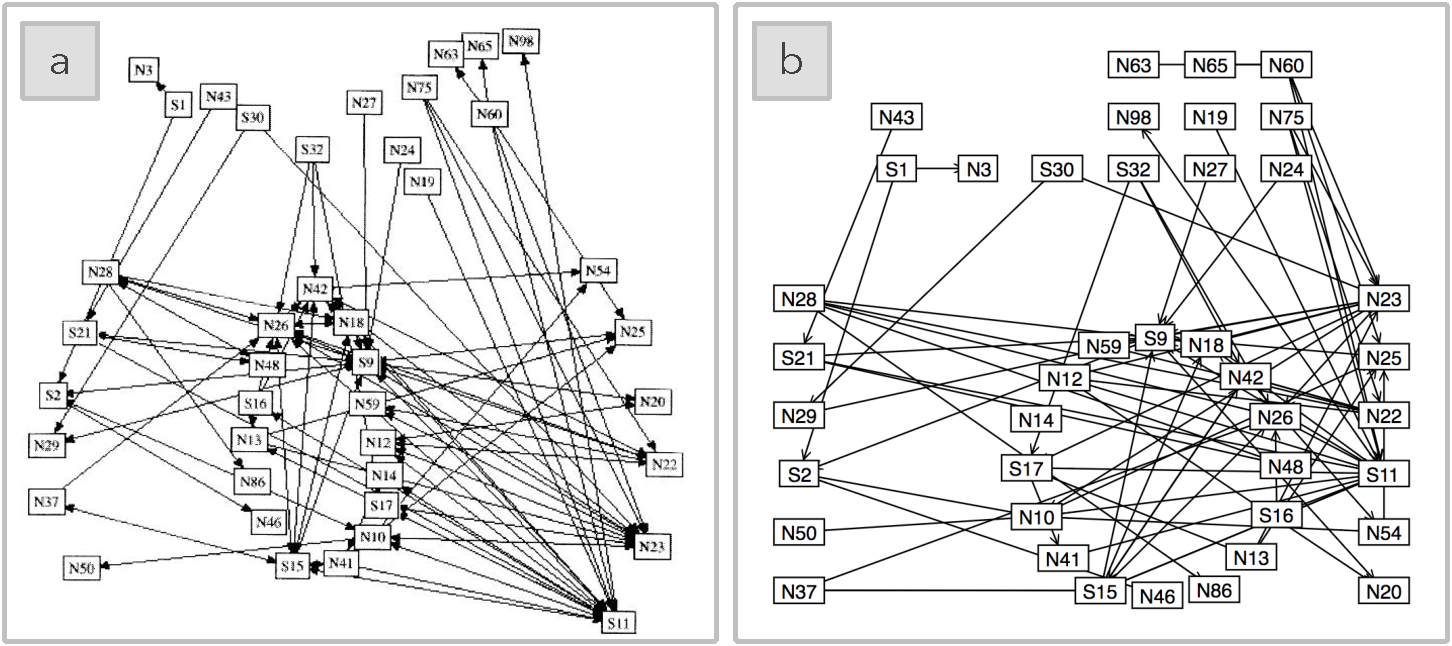
\includegraphics[width=\textwidth]{figures/syphilis-layout.pdf}
    \vspace{-20px} {\caption{\label{fig:syphilis-layout} The layout for the
        syphilis social network from (a) Rothenberg et
        al.~\cite{rothenberg1998using}. (b) We recreated and improved the
        layout in \projectname by introducing additional padding, alignment,
        and circle constraints to further highlight the \emph{``intensity of interaction''}
        amongst ethnographic groups. For both figures, the nodes are split
        into ethnographically definable groups, from left to right: affluent 
        white men, young white women, and African-American men. Individuals
        not associated with any of these ``core'' groups are positioned above 
        the others.}}
  \end{figure*}
}

\newcommand{\syphilisSpec}{
  \begin{figure}[t]
    \centering
    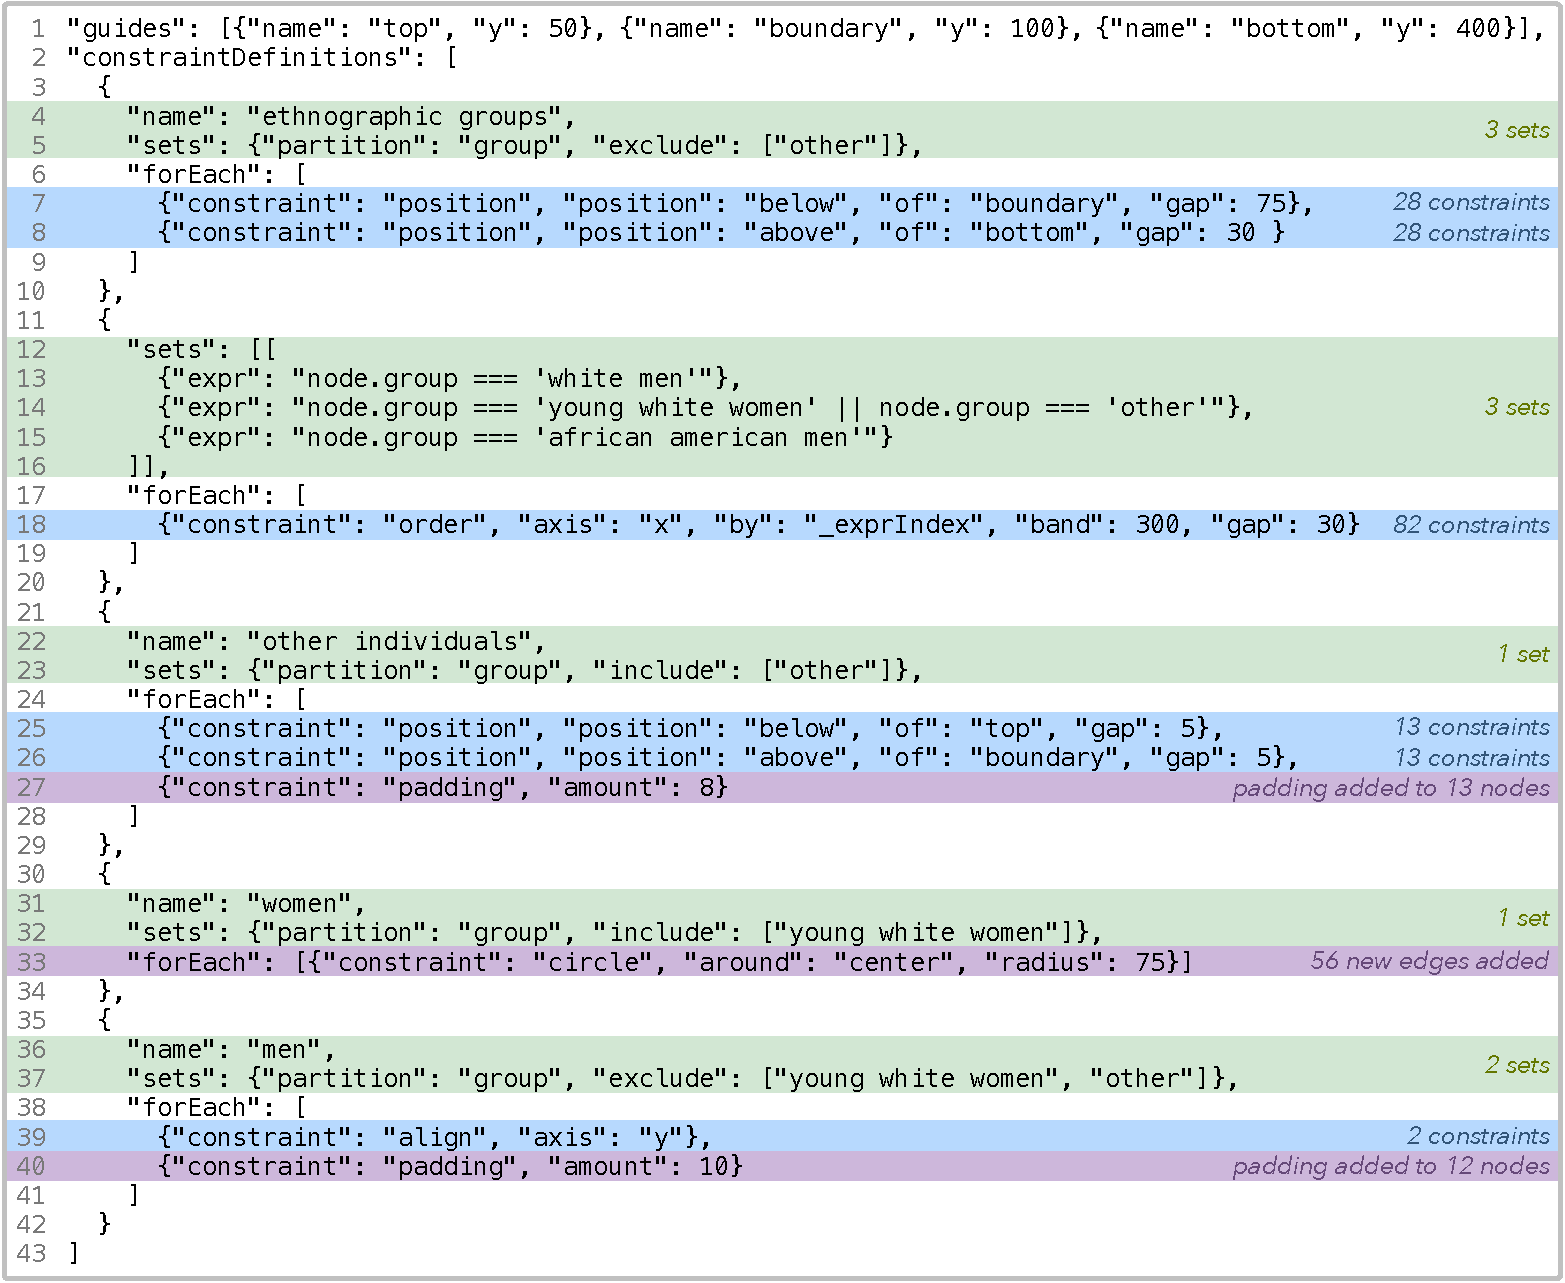
\includegraphics[width=\columnwidth]{figures/syphilis-spec.pdf}
    \vspace{-20px} {\caption{\label{fig:syphilis-spec} The
        \projectname~specification for the syphilis social network shown in
        Figure~\ref{fig:syphilis-layout}. The code is annotated with the
        number of sets produced (green), the number of WebCoLa constraints
        generated for the final layout (blue), and the behavior of \projectname
        constraints \emph{not} converted to WebCoLa (purple).
    }}
  \end{figure}
}

\newcommand{\tlrfourLayout}{
  \begin{figure}[t!]
    \centering
    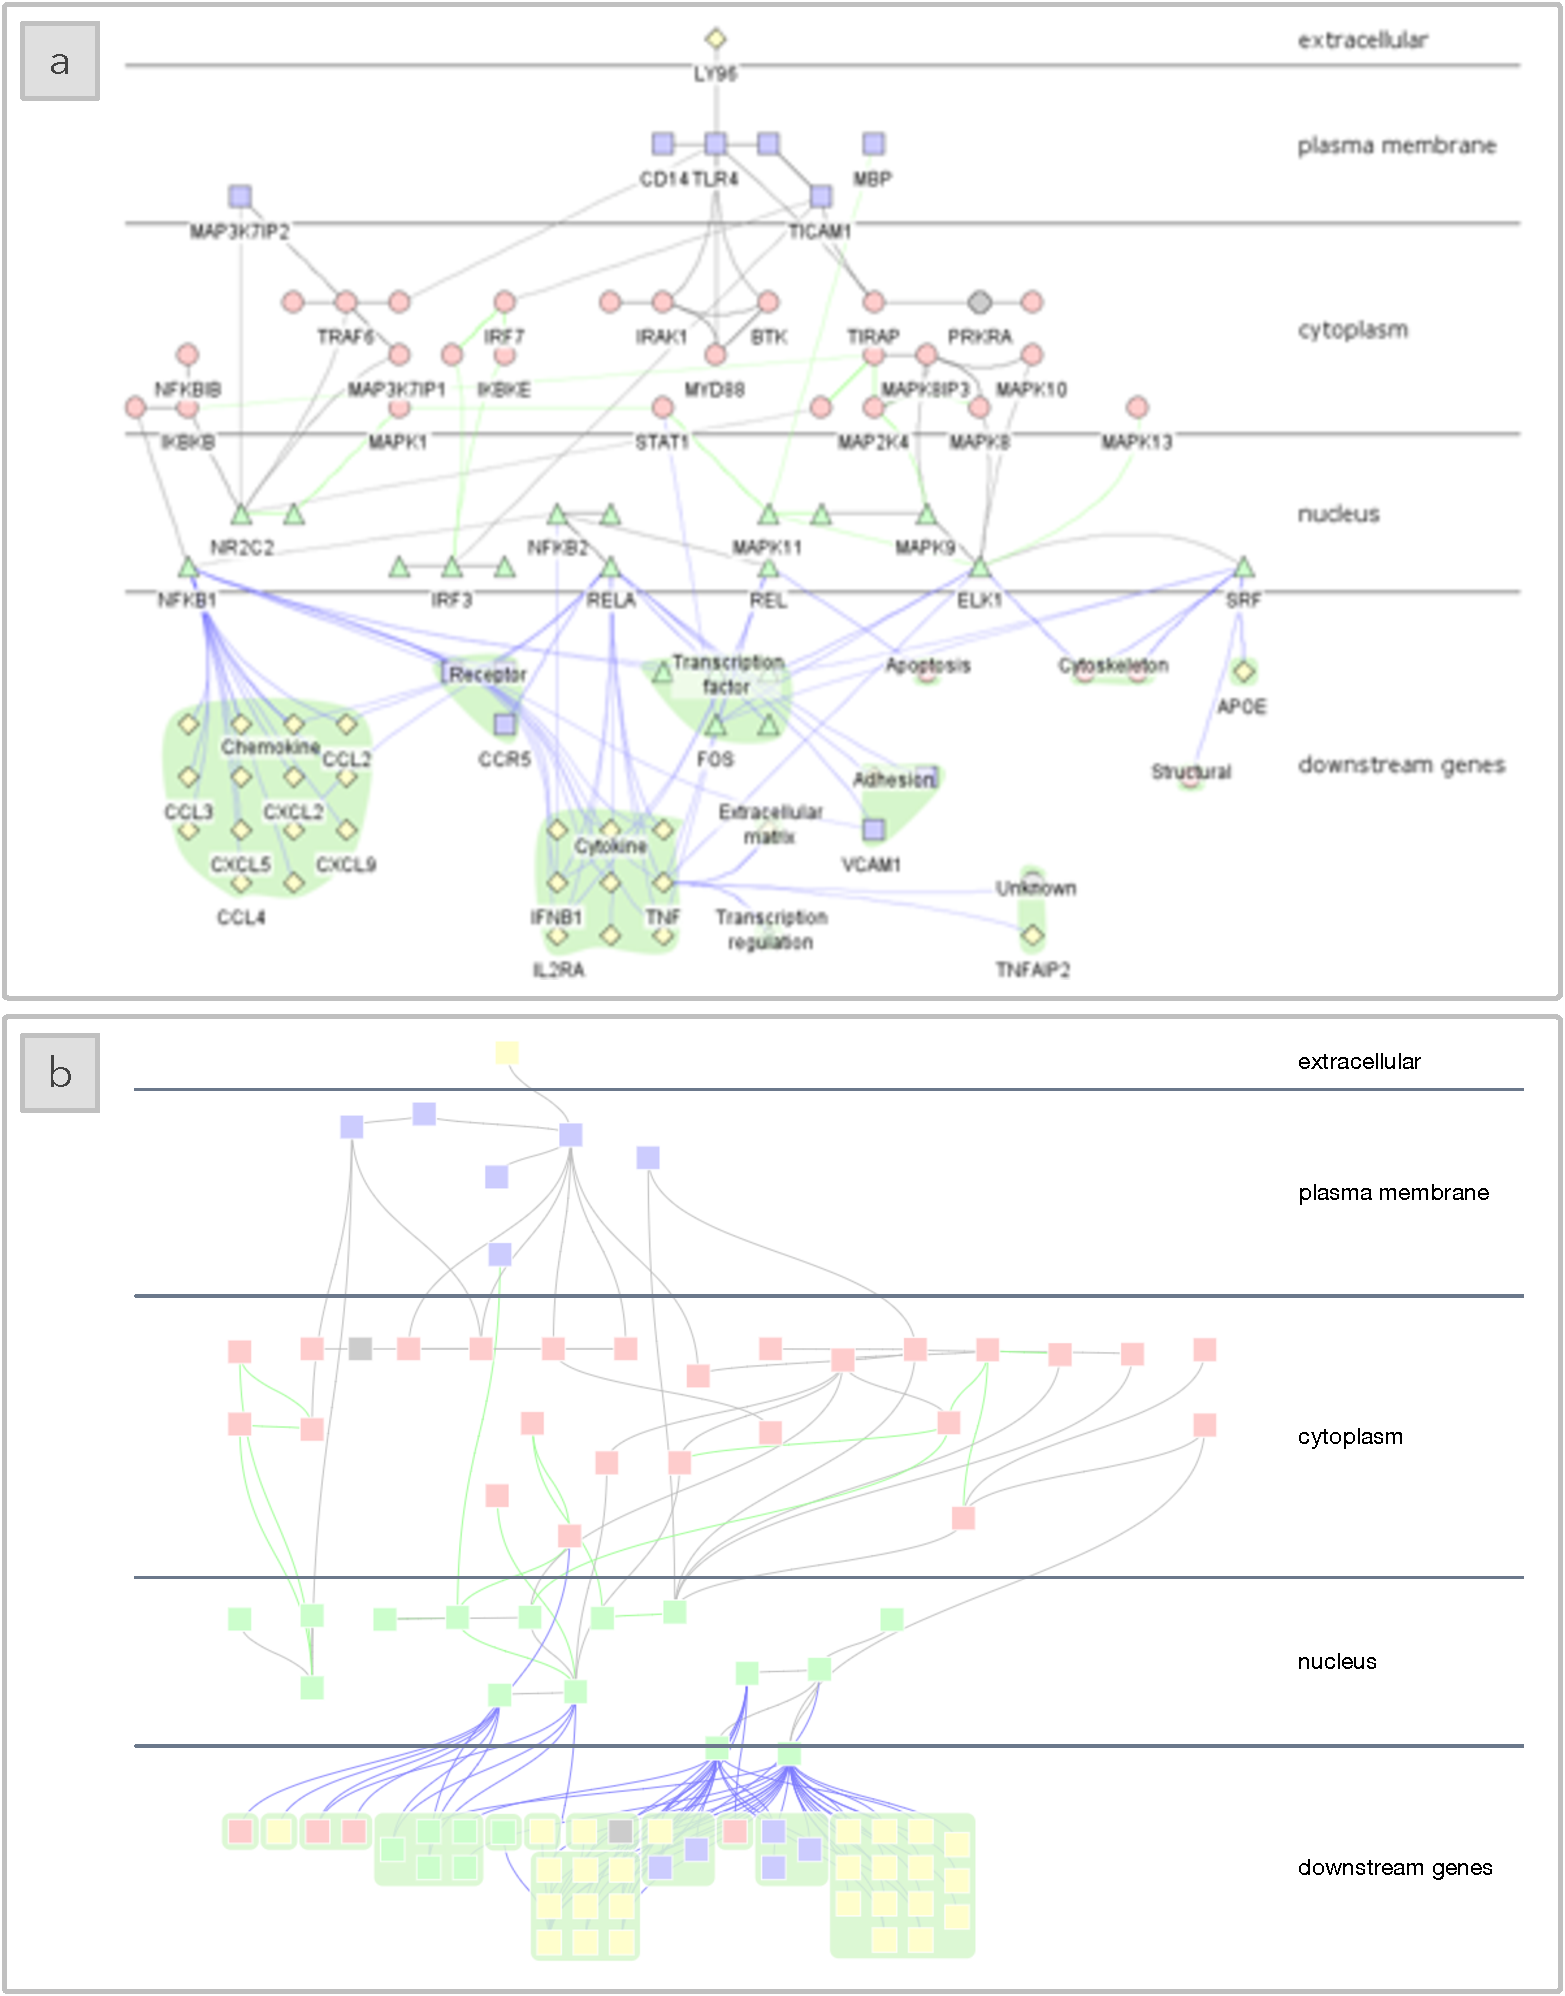
\includegraphics[width=\columnwidth]{figures/tlr4-layout.pdf}
    \vspace{-10px} {\caption{\label{fig:tlr4-layout} The layout for
        the TLR4 biological system produced using (a) Cerebral~\cite{barsky2008cerebral},
        a domain-specific layout tool, as compared to (b) \projectname.
    }}
    \vspace{-30px}
  \end{figure}
}

\newcommand{\tlrfourSpec}{
  \begin{figure}[t]
    \centering
    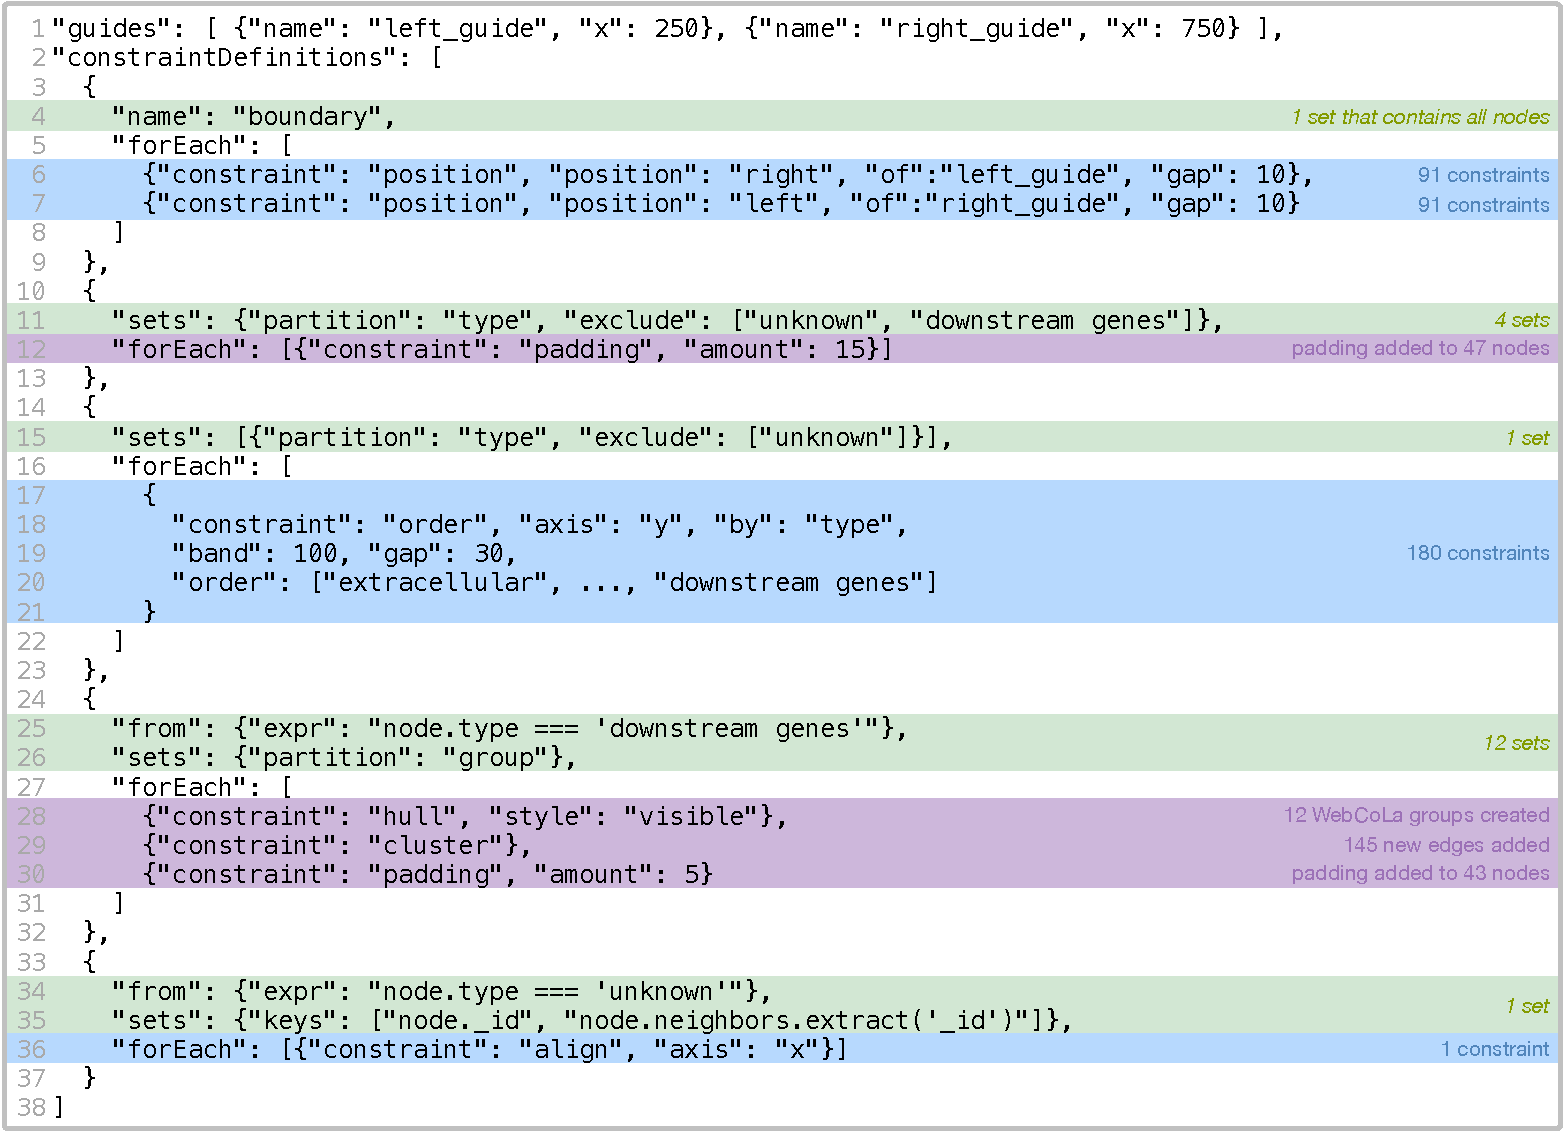
\includegraphics[width=\columnwidth]{figures/tlr4-spec.pdf}
    \vspace{-20px} {\caption{\label{fig:tlr4-spec} The
        \projectname~specification for the TLR4 biological system shown in
        Figure~\ref{fig:tlr4-layout}.
        \feedback{Younghoon}{I could infer what ``from'' and ``forEach'' 
        mean in TLR4. But hard to infer ``collect''. (I might miss the 
        description for these...).}}}
  \end{figure}
}

\newcommand{\constraintsFigure}{
  \begin{figure*}[t]
    \centering
    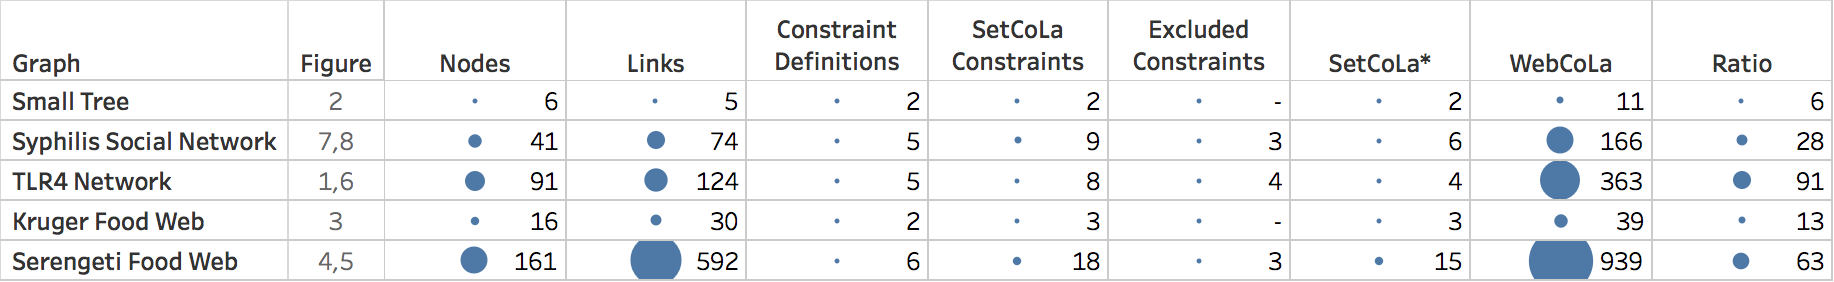
\includegraphics[width=\textwidth]{figures/constraints.png}
    \vspace{-20px} {\caption{\label{fig:constraints}
    The number of nodes, links, and constraints for each example. We show
    the number of constraint definitions and number of \projectname constraints
    written by the user. * Some \projectname constraints are not directly
    converted to WebCoLa, so we also denote the number of these constraints
    (\textbf{Excluded Constraints}) and compare the reduced number (\textbf{SetCoLa})
    to the number of constraints produced in \textbf{WebCoLa}.}}
  \end{figure*}
}